\documentclass[letter, 10pt]{article}
\usepackage[utf8]{inputenc}
\usepackage[spanish]{babel}
\usepackage{amsfonts}
\usepackage{amsmath}
\usepackage[dvips]{graphicx}
\usepackage{subfigure}
\usepackage{url}
\usepackage[top=3cm,bottom=3cm,left=3.5cm,right=3.5cm,footskip=1.5cm,headheight=1.5cm,headsep=.5cm,textheight=3cm]{geometry}


\begin{document}
\title{Taller de Modelos y Métodos Cuantitativos \\ \begin{Large}Sintonización: Algoritmo \emph{Clonal Selection} para el problema \emph{Car Sequencing Problem}\end{Large}}
\author{Cristián D. Maureira Fredes.}
\date{\today}
\maketitle

\section{Introducción}
\frame
{
\frametitle{Introducción}
\begin{itemize}
	\item Motivación del problema.
	\item Sobre la técnica.
	\item Implementación inicial.
	\item Sintonización.
	\item \blue{Control}.
	\item Resultados.
\end{itemize}
}



\section{Sintonización}

\subsection{Parámetros del algoritmo}
%Definición y análisis de cada uno de los parámetros que posea su algoritmo. \\
%
%Ej. \textit{Temperatura (Simulated Annealing); [0,1] parámetro que define la probabilidad con la cual se aceptan soluciones de peor calidad en cada iteración. Un valor alto para este parámetro involucra una fuerte e exploración, en cambio valores bajos indican una inclinación a la explotación.} \\
%Puede incluir diagramas o todo lo que sea necesario para dejar claras las caracteristicas y función que cumple el parámetro en su algoritmo.

\begin{itemize}
	\item \texttt{POP} \blue{[10,210]}, Parámetro que define el tamaño de cada población al momento de comenzar
			las iteraciones a través de la cantidad de generaciones.
			Este parámetros influye notablemente en el tiempo que demora la ejecución de nuestro algoritmo,
			pues si tenemos poblaciones muy grandes todo el tratamiento que le damos a los individuos,
			como la hipermutación y la clonación tomará mucho más tiempo.

	\item \texttt{GENS} \blue{[10,2000,30]}, Parámetro que define el número total de generaciones en las cuales
			el algoritmo se mantendrá en ejecución. Este parámetro es la actual condición de término
			por lo cual es esencial a la hora de obtener buenos o malos resultados, ya que si tenemos
			muy pocas generaciones, para muchas variables puede que no se alcance a cumplir bien los
			objetivos del algoritmo y que se termine no con los mejores resultados.

	\item \texttt{clonationFactor} \blue{[0,1]} \red{$(\beta)$}, Parámetro que sirve para definir la cantidad de clones
			que vamos a generar a partir de un elemento anteriormente seleccionado, considerando la
			fórmula propuesta por De Castro~\cite{decastro}, en el cual consideramos tres elementos:
			``factor de clonación ($\beta$)'', ``Total de anticuerpos($N$)'' y ``Afinidad (ranking) ($a$)''.
			
			La relación está dada por un número $m$ que equivale a la cantidad de clones que se generarán
            para cada anticuerpo ordenados por afinidad, partiendo del mejor al peor:

            $$m\ =\ \left\lceil\frac{\beta \cdot N}{a}\right\rceil$$

            Con ésto estamos siguiendo la idea central del algoritmo, pues estamos favoreciendo a que se clonen más
            los mejores elementos de nuestra población.

			Adicionalmente, cabe señalar que es posible considerar un $\beta > 1$, dependiendo del nivel
			de clonación que estemos interesados en utilizar.

	\item \texttt{clonationRate}   \blue{[0,1]}, Parámetro que define la cantidad de elementos que seleccionaremos
			para poder comenzar el proceso de clonación. Aquí se seleccionan \texttt{POP*clonationRate} elementos
			de una población que ya se encuentra ordenada de acuerdo al \emph{fitness}, es decir, de los mejores
			a los peores, por lo tanto nos aseguramos de que las futuras clonaciones sean a buenos individuos.

	\item \texttt{replaceRate}     \blue{[0,1]}, Parámetro que define la cantidad de nuevos elementos que
			integramos en nuestra población para poder así combatir el estancamiento en óptimos locales,
			de ésta forma se generan una cantidad de \texttt{POP*replaceRate} nuevos individuos, en las posiciones
			de los peores elementos, siendo éste el mecanismo para tener variación en nuestra población.

\end{itemize}


\subsection{Sintonización Manual}
%Se deben explicar todas las pruebas de sintonización manual realizadas. Para esto debe usar la estructura que se adjunta abajo.\\

Para la presente sección, se requiere de una configuración inicial,
para poder comenzar a evaluar el rendimiento del algoritmo para
cada situación donde se quiera sintonizar manualmente algún parámetro.

Los valores de la configuración inicial están dado en base a la experiencia
del trabajo pasado, es decir, en la \emph{primera implementación}.

\begin{itemize}
	\item \texttt{POP = 20}
	\item \texttt{GENS = 200}
	\item \texttt{clonationFactor = 0.4}
	\item \texttt{clonationRate = 0.5}
	\item \texttt{replaceRate = 0.6}
\end{itemize}

Complementariamente, se han considerado tres instancias provenientes de la CSPlib~\cite{CSP}
más precisamente de la sección \emph{``30 new hard problems from Caroline Gagne ''},
donde se han escogido tomando en cuenta el mejor resultado encontrado.
Las instancias son:

\begin{center}
	\begin{tabular}{|l|c|}
	\hline
	\textbf{Instancia} & \textbf{Mejor resultado conocido} \\\hline
	\texttt{pb\_200\_01.txt} & 0 \\\hline
	\texttt{pb\_200\_09.txt} & 10 \\\hline
	\texttt{pb\_200\_10.txt} & 19 \\\hline
	\end{tabular}
\end{center}
\newpage
\subsubsection{Tamaño de población}

\textbf{Prueba}: \blue{prueba1}\\

\textbf{Parámetros involucrados:} Tamaño de población \texttt{(POP)}.\\

\textbf{Objetivo:} Analizar el comportamiento de acuerdo a fitness y tiempo de ejecución del parámetro en un rango de valores.\\

\textbf{Metodología:} Se probarán varios valores en el rango de valores del parámetro \blue{[10,210]}.\\

\textbf{Gráfico:}\\

\begin{figure}[h!]
\begin{center}
	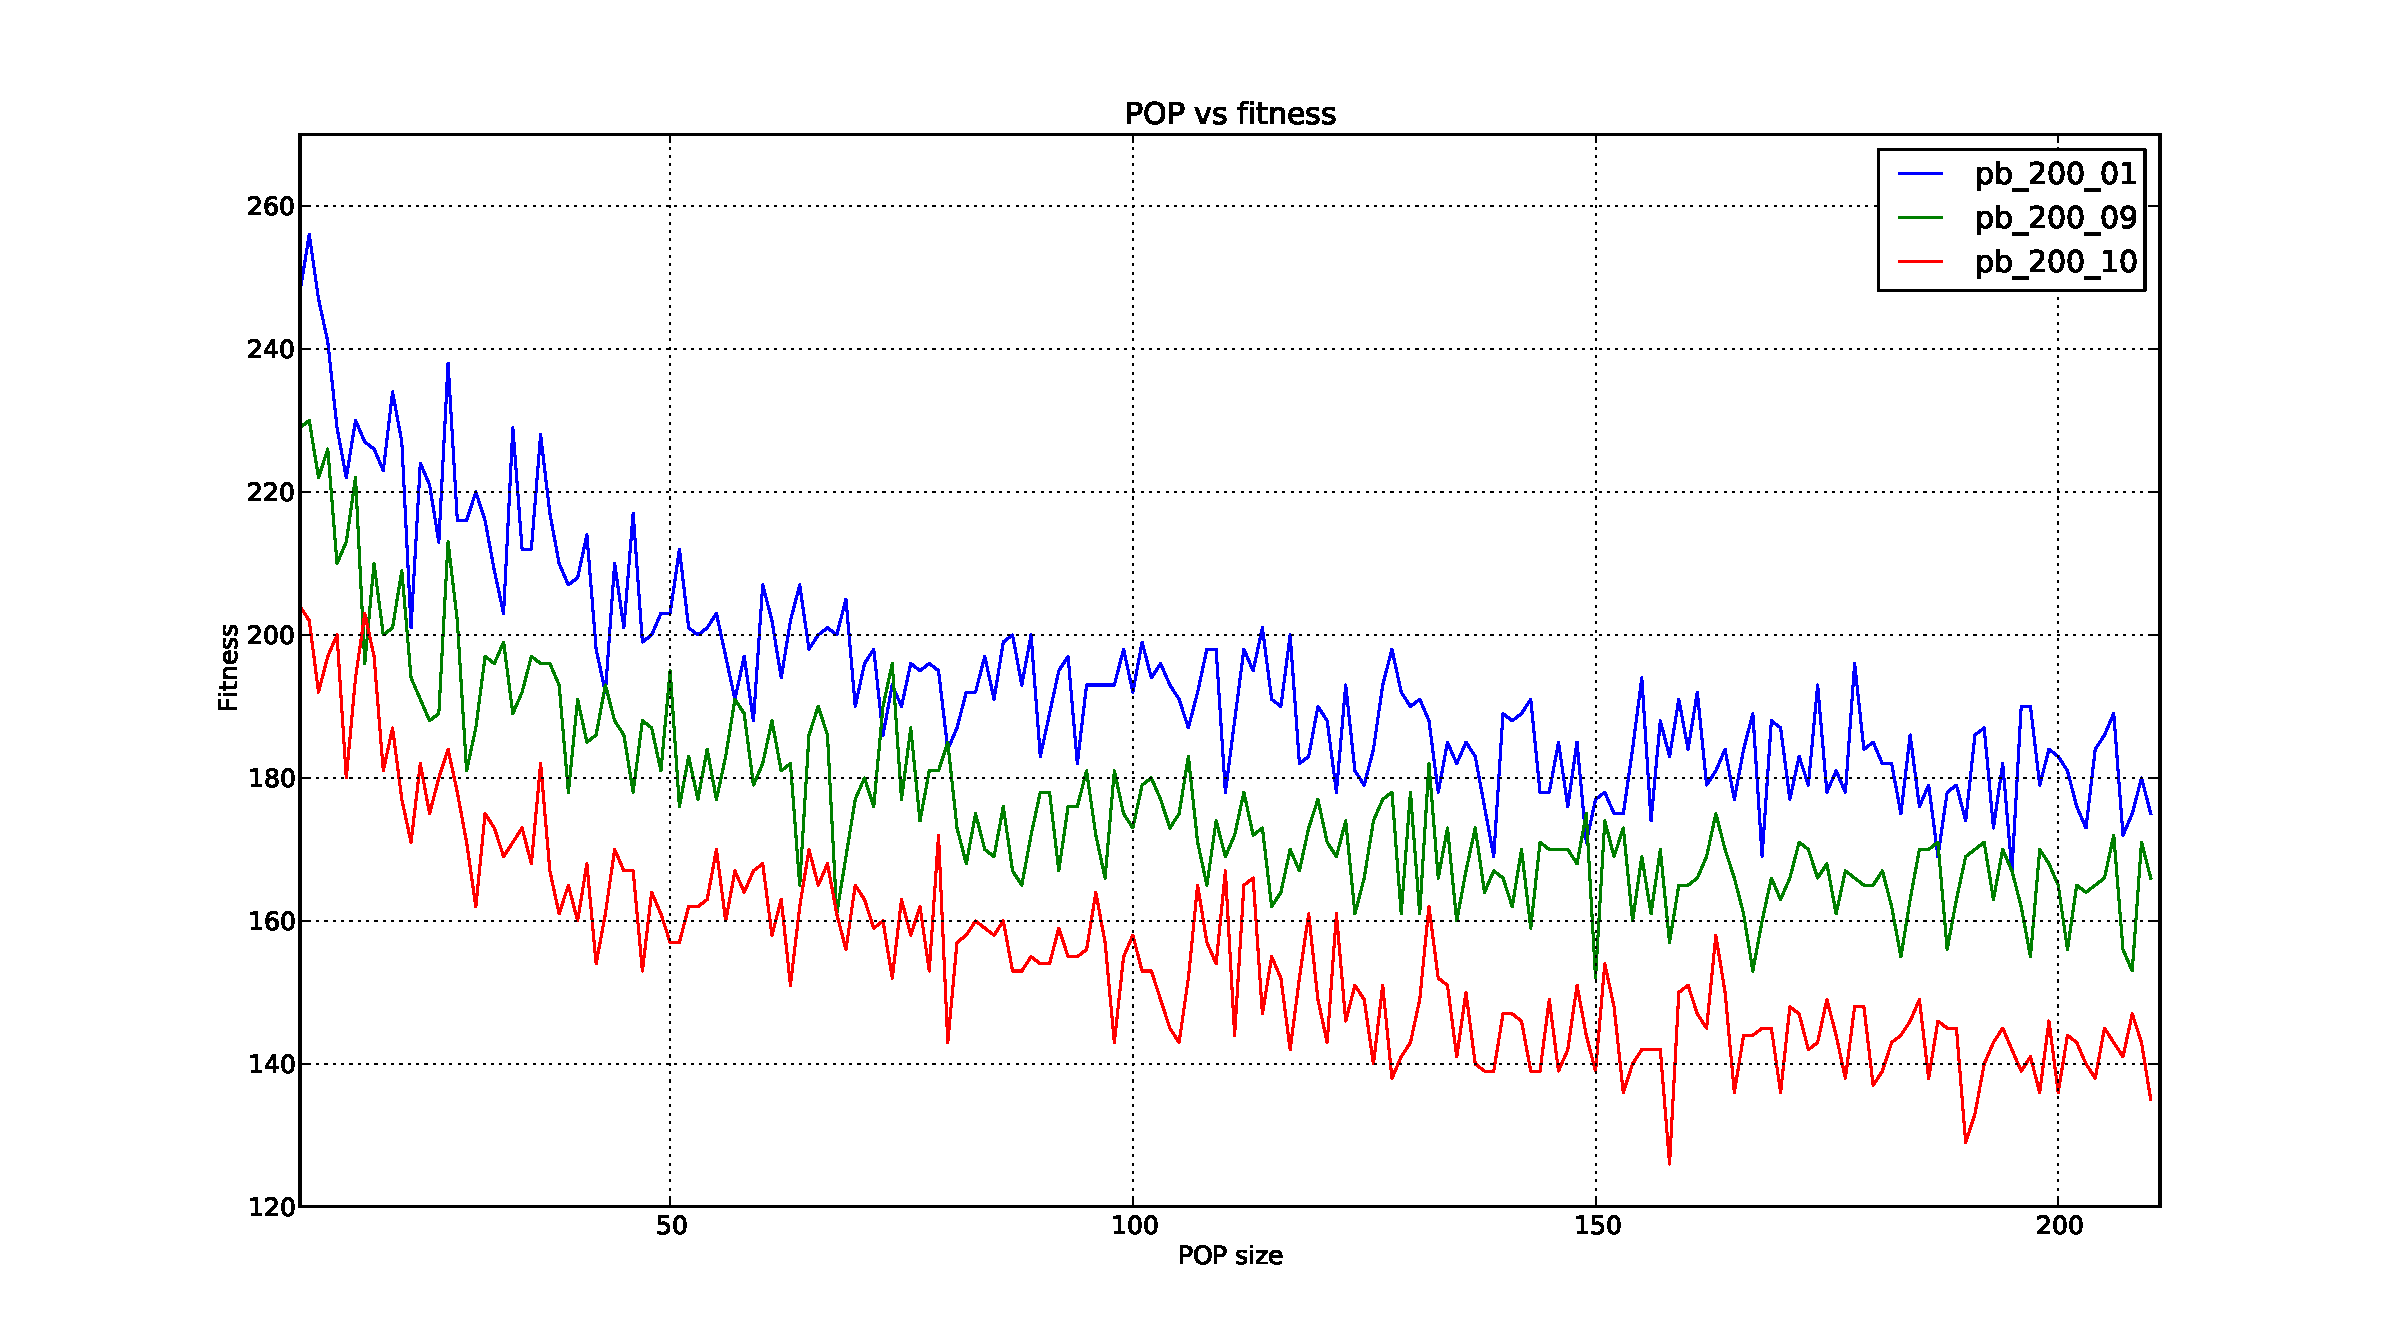
\includegraphics[width=0.95\textwidth]{img/1.pdf}
	\caption{Comparaci\'on de las tres instancias dado un cambio en la poblaci\'on}
	\label{fig:1}
\end{center}
\end{figure}

\textbf{Configuración escogida:}\\

La siguiente tabla, proporciona la información pertinente del mejor resultado obtenido,
de las $200$ iteraciones en las que consistió la presente prueba por cada instancia.

Gracias a la figura~\ref{fig:1}, podemos darnos cuenta del comportamiento que nuestro
algoritmo va teniendo a medida que vamos aumentando el tamaño de la población.

En un comienzo podemos ver el pésimo comportamiento que posee, pues como la cantidad de
la población es muy pequeña, los anticuerpos no van a poder variar mucho, ya que al
momento de clonar o introducir diversidad, no cumplen su objetivo principal, pues
como estos procedimiento van a depender netamente del tamaño de la población, no serán
del todo útiles.

Cabe señalar que en realidad el comportamiento que está tomando el algoritmo, es más
bien siempre trabajar con soluciones aleatorias, pues la hipermutación de los clones
está determianda por el índice de la población, por lo que el mayor individuo se mutará
muy poco, lo que llevará a obtener pocas mejoras en nuestros anticuerpos.


\begin{center}
\begin{tabular}{|l|c|c|c|c|}
	\hline
	\textbf{Instancia} & \textbf{POP} & \textbf{Mejor resultado} & \textbf{Tiempo [s] } & \textbf{Tiempo total [s] }\\\hline
	\texttt{pb\_200\_01.txt} & 195 & 167 & 15.110 & 1608.853 \\\hline 
	\texttt{pb\_200\_09.txt} & 150 & 152 & 11.243 & 1593.739 \\\hline
	\texttt{pb\_200\_10.txt} & 158 & 126 & 11.210 & 1662.580 \\\hline
\end{tabular}
\end{center}

Las iteraciones luego de un tamaño en la población sobre $100$ aproximadamente,
se comienzan a comportar de una forma más normalizada, y la pendiente de la curva que aproxima
al comportamiento del algoritmo, se vuelve cada vez menor, lo cual está representado en la tabla,
ya que claramente los mejores rendimientos por cada instancia están sobre una población de
tamaño $100$.

A pesar de lo distinta que son cada instancia, en nivel de complejidad, los tiempos que toman
cada una están bien parecidas, entre $11$ y $15$ segundos, por lo que no hay mayor diferencia.
\newpage
\subsubsection{Número de generaciones}

\textbf{Prueba}: \blue{prueba2}\\

\textbf{Parámetros involucrados:} Número de generaciones \texttt{(GENS)}.\\

\textbf{Objetivo:} Analizar el comportamiento de acuerdo a fitness y tiempo de ejecución del número de generaciones entre un rango de valores.\\

\textbf{Metodología:} Se probarán varios valores en el rango de valores del parámetro \blue{[10,2000]} (iterando de 30 en 30).\\

\textbf{Gráfico:}\\

\begin{figure}[h!]
\begin{center}
	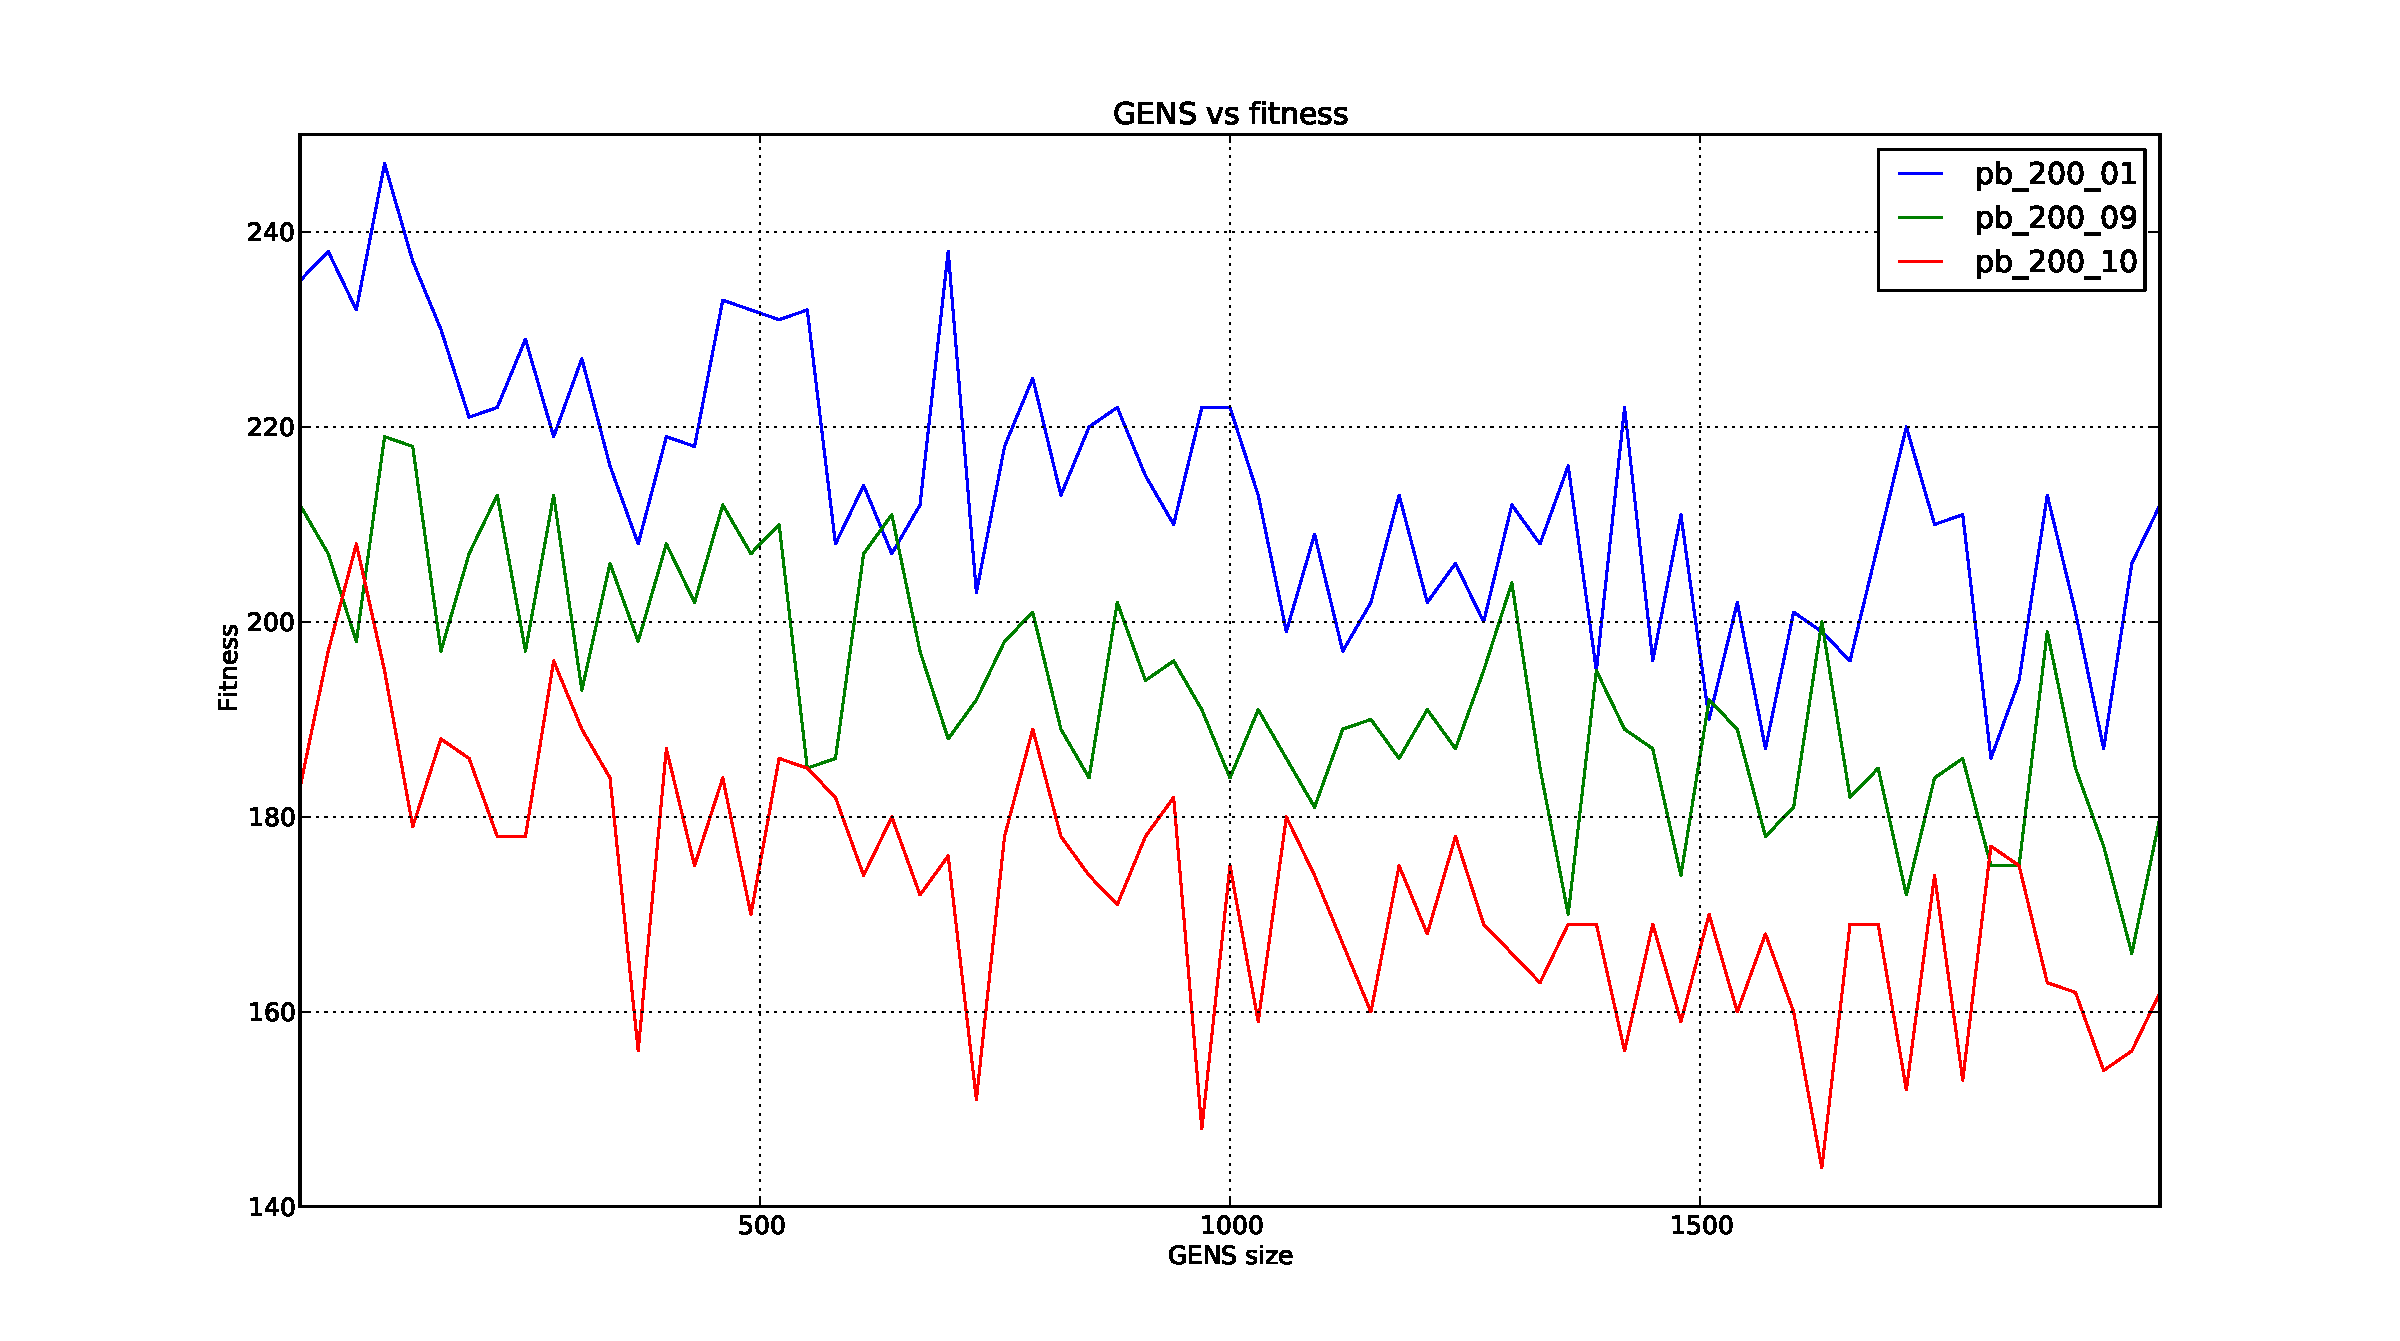
\includegraphics[width=0.95\textwidth]{img/2.pdf}
	\caption{Comparaci\'on de las tres instancias dado un cambio en el n\'umero de generaciones}
	\label{fig:2}
\end{center}
\end{figure}

\textbf{Configuración escogida:}\\

\begin{center}
\begin{tabular}{|l|c|c|c|c|}
	\hline
	\textbf{Instancia} & \textbf{GENS} &\textbf{Mejor resultado} & \textbf{Tiempo [s] } & \textbf{Tiempo total [s]}\\\hline
	\texttt{pb\_200\_01.txt} & 1810 & 186 & 7.782 & 256.177 \\\hline
	\texttt{pb\_200\_09.txt} & 1960 & 166 & 8.460 & 262.906 \\\hline
	\texttt{pb\_200\_10.txt} & 1630 & 144 & 7.562 & 256.546 \\\hline
\end{tabular}
\end{center}

\newpage
\subsubsection{Tasa de reemplazo}

\textbf{Prueba}: \blue{prueba3}\\

\textbf{Parámetros involucrados:} Tasa de reemplazo \texttt{(replaceRate)}.\\

\textbf{Objetivo:} Analizar el comportamiento de acuerdo a fitness y tiempo de ejecución de la tasa de reemplazo entre un rango de valores.\\

\textbf{Metodología:} Se probarán varios valores en el rango de valores del parámetro \blue{[0,1]}.
Para éste caso en particular, se ejecutó el algoritmo 10 veces por cada valor del parámetros y luego se seleccionó la mejor
para poder hacer el siguiente análisis.\\

\textbf{Gráfico:}\\

\begin{figure}[h!]
\begin{center}
	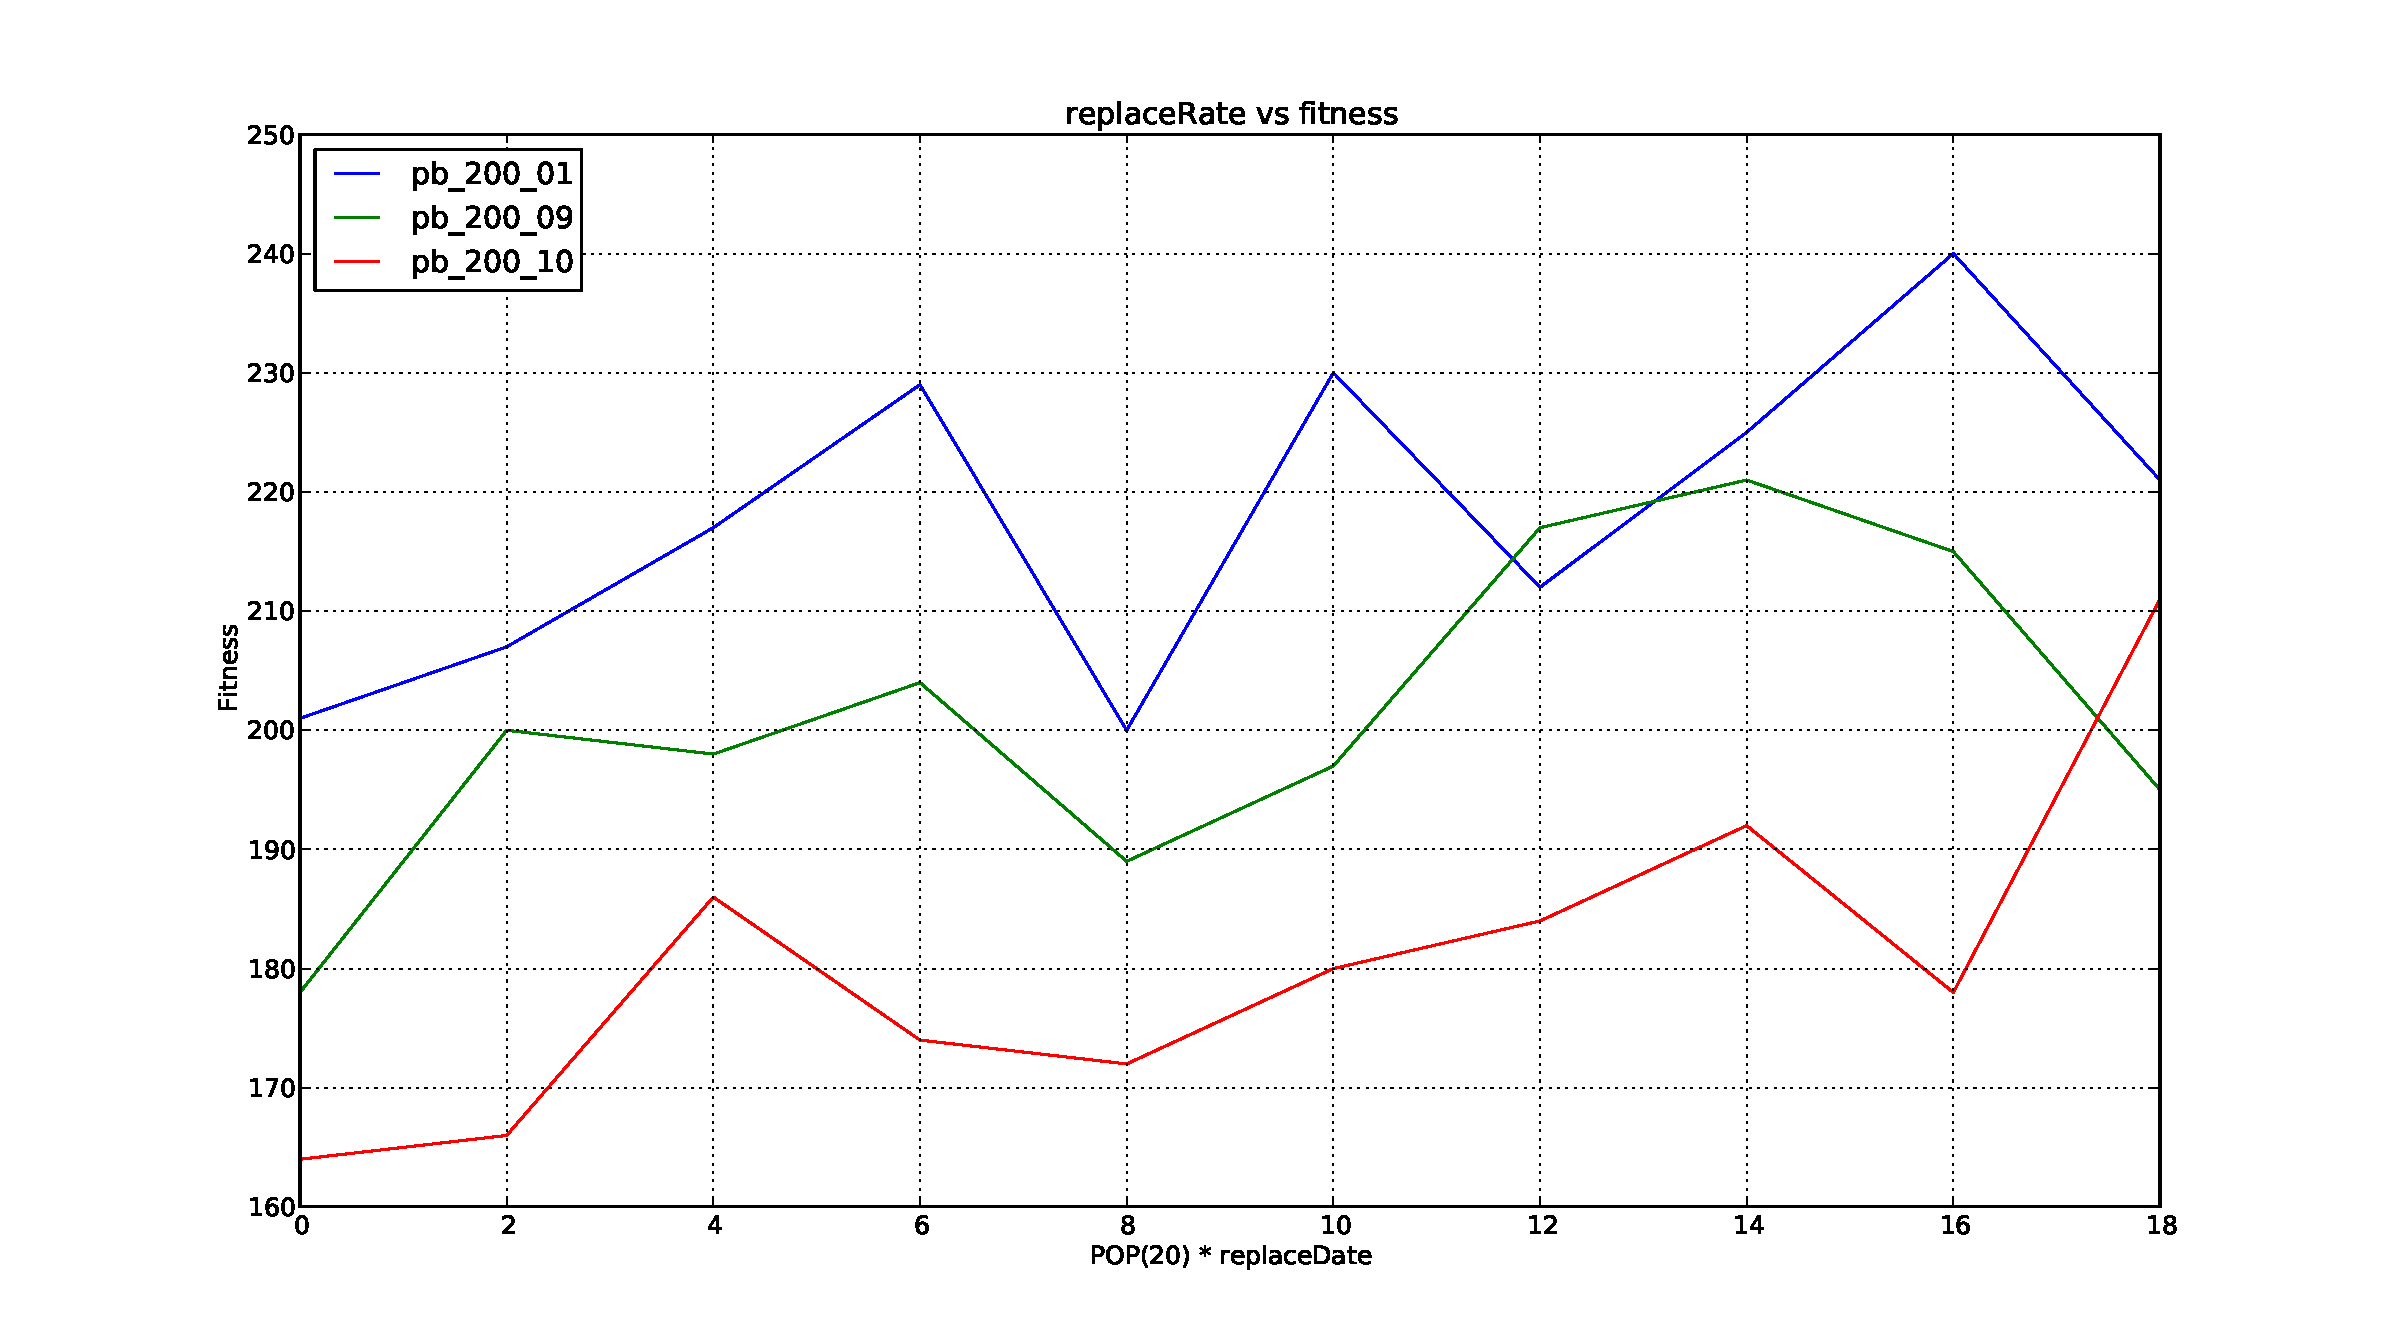
\includegraphics[width=0.95\textwidth]{img/3.pdf}
	\caption{Comparaci\'on de las tres instancias dado un cambio en la tasa de reemplazo}
	\label{fig:3}
\end{center}
\end{figure}

\textbf{Configuración escogida:}\\

La siguiente tabla, proporciona la información pertinente del mejor resultado obtenido,
de las $100$ iteraciones en las que consistió la presente prueba por cada instancia.

En éste caso, como se probaba la ``Tasa de reemplazo'' los valores posible son $0.1, 0.2, \ldots, 1.0$,
por lo que se realizó $10$ pruebas por cada valor.

Gracias a la figura~\ref{fig:3} nos podemos dar cuenta que los mejores valores se encuentran
para valores pequeños de la ``Tasa de reemplazo'' para las dos instancias finales, en cambio
para la primera instancia es un valor de $0.4$.

Podríamos ingenuamente decir, nuestro algoritmo no necesita ingresar diversidad y que por lo tanto
sólo nos dedicamos a \emph{explotar}, pero los resultados obtenidos se deben a que las iteraciones
que utilizamos como configuración básica son muy pocas, son sólo $200$, por lo que nuestro algoritmo
no alcanza a desarrollarse para poder tener la necesidad de salir de los ``óptimos locales'',
y así poder necesitar insertar diversidad, es por ésto que los valores de las dos últimas instancias,
es 0, pues el algoritmo no alcanza a necesitar diversidad.

\begin{center}
\begin{tabular}{|l|c|c|c|c|}
	\hline
	\textbf{Instancia} & \textbf{POP*replaceRate} & \textbf{Mejor resultado} & \textbf{Tiempo [s]} & \textbf{Tiempo total [s]}\\\hline
	\texttt{pb\_200\_01.txt} & 8 & 200 & 1.374 & 13.246 \\\hline
	\texttt{pb\_200\_09.txt} & 0 & 178 & 1.463 & 12.027 \\\hline
	\texttt{pb\_200\_10.txt} & 0 & 164 & 0.515 & 12.133   \\\hline
\end{tabular}
\end{center}


\newpage
\subsubsection{Factor de clonación y Tasa de clonación}

\textbf{Prueba}: \blue{prueba4} \\

\textbf{Parámetros involucrados}: Tasa de clonación y Factor de clonación. \\

\textbf{Objetivo}: Estudiar el efecto de la tasa y el factor de clonación en conjunto de acuerdo a fitness obtenido para la variación
de los dos parámetros en todo tu dominio.\\

\textbf{Metodología}: Se prueban varias combinaciones de valores para ver el efecto de los parámetros y poder observar su comportamiento.\\

\textbf{Configuración escogida:}\\

\begin{small}
\begin{center}
\begin{tabular}{|l|c|c|c|c|c|}
	\hline
	\textbf{Instancia} & \textbf{clonationRate} & \textbf{clonationFactor} &\textbf{Mejor resultado} & \textbf{Tiempo [s]} & \textbf{Tiempo total [s]}\\\hline
	\texttt{pb\_200\_01.txt} & 0.6 & 1   & 192 & 1.241 & 132.608 \\\hline
	\texttt{pb\_200\_09.txt} & 0.6 & 1   & 180 & 1.378 & 132.068 \\\hline
	\texttt{pb\_200\_10.txt} & 0.5 & 0.9 & 160 & 1.379 & 132.124 \\\hline
\end{tabular}
\end{center}
\end{small}
\normalsize
\textbf{Gráfico:}\\

\begin{figure}[h!]
\begin{center}
	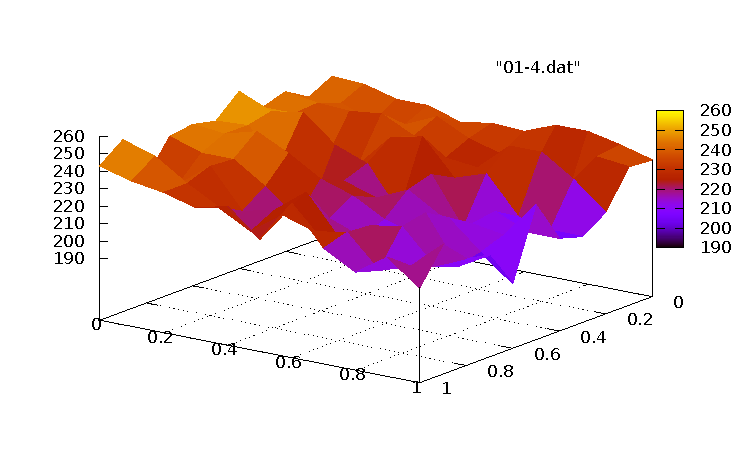
\includegraphics[width=0.95\textwidth]{img/01-4.pdf}
	\caption{Comparaci\'on de la instancia \texttt{pb\_200\_01.txt} variando \texttt{clonationRate} y \texttt{clonationFactor}}
	\label{fig:4-1}
\end{center}
\end{figure}

\begin{figure}[h!]
\begin{center}
	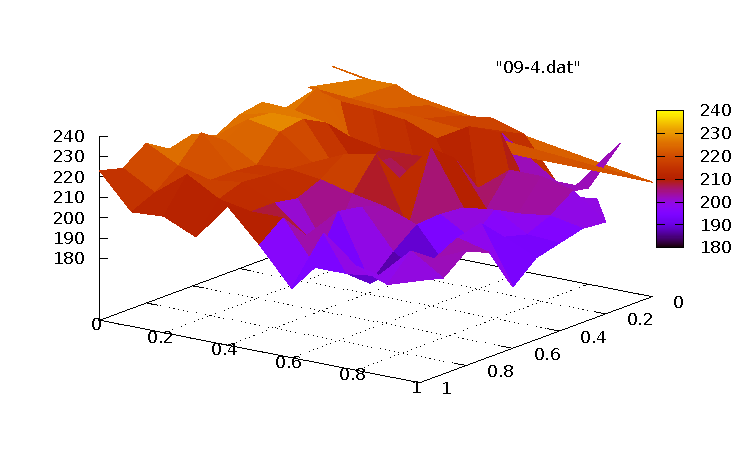
\includegraphics[width=0.95\textwidth]{img/09-4.pdf}
	\caption{Comparaci\'on de la instancia \texttt{pb\_200\_09.txt} variando \texttt{clonationRate} y \texttt{clonationFactor}}
	\label{fig:4-2}
\end{center}
\end{figure}

\newpage 
\begin{figure}[h!]
\begin{center}
	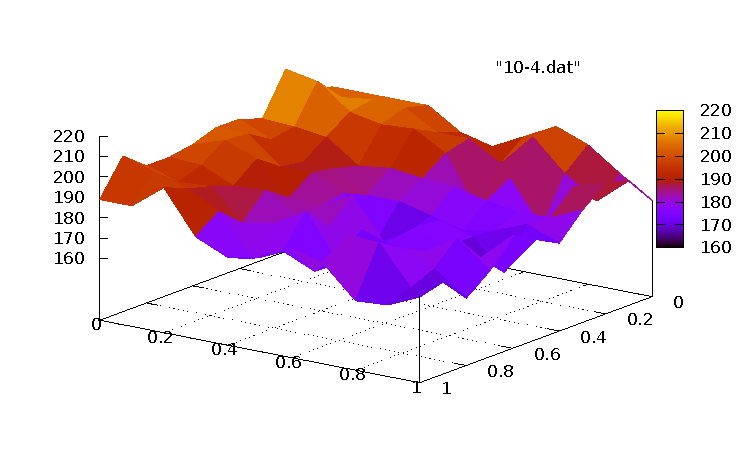
\includegraphics[width=0.95\textwidth]{img/10-4.pdf}
	\caption{Comparaci\'on de la instancia \texttt{pb\_200\_10.txt} variando \texttt{clonationRate} y \texttt{clonationFactor}}
	\label{fig:4-3}
\end{center}
\end{figure}


\newpage
%
%
%elegir una configuración para cada instancia
%	-indicar el fitness
%	-identificar claramente las características del algoritmo.
%	-estimación del tiempo en realizarla.


\subsection{Sintonización Automática}
\frame
{
\frametitle{Sintonización Automática}
\begin{itemize}
	\item 
\end{itemize}
}


\section{Conclusiones}
%De acuerdo a la introducci\'on que se hizo, entregar afirmaciones
%  basadas en los experimientos y sus resultados.

A primera vista, los resultados obtenidos en la presente implementación, superan en gran medida a los óptimos encontrados
en todos estos años, donde distintas personas, han utilizado, variadas técnicas para poder resolver el \emph{Car Sequencing Problem}
de la mejor manera, considerando así, que se pudieron haber utilizado técnicas completas, que si bien es cierto, pueden demorar mucho,
van a encontrar el \emph{óptimo global} de un determinado problema, lo cual se diferencia notoriamente con las técnicas incompletas,
como es el caso de ka presente implementación, donde sólo se puede encontrar un \emph{óptimo local}.

Al mirar el gráfico podemos darnos cuenta, de que la distribución de la cantidad de restricciones violadas, poseen un comportamiento
bastante similar, guardando las proporciones de la cantidad de violaciones, lo que nos hace deducir, de que sólo nos falta un poco
más de control y sintonización de los parámetros utilizados, para acercarnos aún más a soluciones más óptimas.

Siguiendo con el análisis de los experimentos, podemos darnos cuenta de que si bien es cierto, las soluciones violan una cantidad
considerable de restricciones, estamos sacrificando una buena solución, por un corto tiempo de ejecución, el cual en algunos casos,
sólo llega a durar 1 minuto, lo que comparado con el tiempo de alguna técnica completa, que puede durar días, nos beneficia de cierta manera.

Con respecto a la representación del problema, existen ciertos pros y contras.
Primero que todo la representación que se utilizó en la presente implementación,
consiste en una del tipo no-binaría, por lo que no es tan fácil utilizar los típicos movimientos de las representaciones binarias,
como lo son el \emph{bit-flip} y el \emph{cruzamiento en un punto}, ya que estaríamos violando las restricciones duras del problema,
por lo cual en la presente implementación, por ejemplo, no se utilizó un operador de cruzamiento y sólo se deposito la confianza,
en la mutación con \emph{Simulated Annealing} que se encargó tanto de explorar como de explotar.

Según lo anteriormente dicho, el no poseer un operador de cruzamiento, puede haber perjudicado la explotación del presente algoritmo
evolutivo, y por ende, entorpecido la búsqueda de un óptimo local. Aunque los resultados no fueron del todo malos, por lo que el simulated annealing
hizo su trabajo explorando y explotando, pero no de la forma más apropiada.

Otro punto importante en la presente implementación, es la forma en la cual se genera la población inicial.
Como ya hemos mencionado anteriormente, lo favorable del método utilizado es que se generan soluciones factibles,
es decir, que cumplen las restricciones duras, pero por otro lado, éstas se generan de forma aleatoria, lo cual indica,
que quizás utilizando alguna técnica de construcción de individuos más apropiada, como Greedy o GRASP, la calidad de la
población inicial aumentaría, lo cual sería interesante como trabajo futuro.


Con respecto a la mutación con simulated annealing, cabe señalar que existen algunos aspectos que pueden ser mejorados,
como por ejemplo un control de la temperatura, pues en la presente implementación, la temperatura disminuye cada 3 iteraciones,
lo que si tomamos en cuenta un control más riguroso, como comparar la calidad de las soluciones generadas, podríamos
realizar los cambios en la temperatura, a medida que el algoritmo se comporta de una forma más apropiada.


Finalmente, es posible mejorar la presente implementación de un algoritmo evolutivo aumentando la exploración,
que en éste caso significa poder mejorar lo que es la mutación, ya que dentro del simulated annealing, el movimiento
no es muy apropiado, y quizás el sólo hecho de mejorar el movimiento de la mutación simulated annealing, puede
traer un mejor desempeño en nuestro algoritmo. Otra forma podría ser cambiar el método de la ruleta, pues si bien es cierto,
le entrega una mayor probabilidad para escoger los mejores individuos, no nos prohibe elegir malos individuos, lo que
perjudica a nuestra siguiente población, y por ende a la solución del problema.


% OLD

%Conclusiones revelantes del estudio realizado.

%En el presente informe se ha dado un estado del arte de un problema muy popular
%en el área de la inteligencia artificial, el \emph{Car Sequencing Problem}, siendo éste
%una variación de otro problema connotado llamado \emph{Job Shop Scheduling}.
%Es tanto la importancia del presente problema, que la \emph{French Society of Operations
%Research and Decision-Making Aid} ha decidido ya hace varios años, comenzar lo que se denomina
%\emph{The ROADEF challenge} cada dos años, teniendo como objetivo central,  permitir a las personas
%que se desarrollan en el área de la industria el presenciar todos los avances y evoluciones
%en el ámbito de la Investigación de Operaciones y Análisis de Decisiones, pero no sólo eso
%sino el poder enfrentar directamente problemas decisionales complejos, que ocurren en la industria.
%Siguiendo la idea anterior, lo importante de éste \emph{Challenge} es que en el 2005, se consideró
%como tema principal el \emph{Car Sequencing Problem} debido a la propuesta que realizó RENAULT,
%por lo cual uno podrá imaginar la cantidad de avances que se produjeron, pues cada participante
%abordaba el problema desde una metodología distinta.
%
%Por otra parte, pareciera que un problema relacionado a \emph{ordenar} un conjunto de vehículos
%para ser ensamblados y así obtener el orden más óptimo, no es una tarea difícil, pero claramente
%debido a la complejidad que otorgan las restricciones y de que es un problema de la vida real,
%presenta un grado de dificultad mayor, lo cual queda reflejado por la cantidad de publicaciones 
%e investigaciones que hay al respecto.
%
%Se dieron a conocer también, tres áreas para atacar el presente problema.
%Por un lado tenemos los métodos heurísticos que como bien sabemos, es prácticamente jugar a la ruleta
%rusa con nuestra investigación, pues la heurística solamente selecciona un objetivo de los dos provenientes
%de la definición, una buena solución o un buen tiempo de ejecución. Pero también se presenta que la heurística
%es un mecanismo confiable para decidir \emph{utilizarlo} como un apoyo, mas que utilizarlo solo.
%
%Siguiendo con los mecanismos planteados, se vieron también los  métodos exactos,
%es decir, técnicas de optimización, donde podemos encontrar la \emph{programación lineal entera},
%\emph{branch and bound} y \emph{local search}, los cuales se dedicaban netamente a construir una
%solución óptima a partir de los datos que el mismo problema nos entrega. El único problema que tienen
%éstas técnicas es que la complejidad temporal va a crecer demasiado con respecto al tamaño de nuestro
%\emph{input} del algoritmo.
%
%Dentro de toda la lectura realizada para las distintas técnicas, pude percatarme que las mejores soluciones
%siempre son variaciones de métodos o tomar dos técnicas como complementarias, por ejemplo uno de los
%mejores resultados fue la combinación de un \emph{Ant Colony Optimization} con una heurística dinámica,
%pues claramente se nos señala que el buen uso de una heurística es crucial, es decir, hay que preocuparse
%de leer los estudios que se han publicado, par ver cual es la combinación más óptima.
%
%Finalmente, es impresionante la cantidad de estudios con respecto a éste problema en particular,
%por lo que podemos darnos cuenta que muchos centros de investigación han dedicado tiempo valioso
%para la resolución óptima del \emph{Car Sequencing Problem}, pero no tanto la versión que se estudió,
%que es la propuesta por Parello~\cite{parello}, sino mas bien al desafío de la ROADEF.


\section{Bibliografía}
Se debe referenciar todo paper citado. En caso de referenciar páginas web, debe incluir fecha.

\end{document} 
